\subsubsection{Produktumfang}
\label{sec:Kap-6.1.3.2}

Die Wahl der Systemgrenze bestimmt, welche Aufgabenbereiche das zu entwickelnde System im späteren Einsatz abdecken muss und welche Aufgaben außerhalb des zu entwickelnden Systems liegen und daher von anderen Systemen, von Prozessen oder Personen geleistet werden müssen. Die Aufgabenbereiche des zu entwickelnden Systems bilden den sogenannten Produktumfang (engl. scope) des Systems. Insofern sind die Bestimmung des Systemkontexts und die Festlegung des Produktumfangs eng verbunden. Es geht bei der Festlegung des Produktumfangs um die Abgrenzung zwischen dem, was das Softwareprodukt leisten soll und dem, was außerhalb seines Aufgabenbereichs liegt.

\begin{figure}[h!]
	\centering
	\vspace{2mm} %%% für Druck
	\vspace{\baselineskip} %%% für Druck
	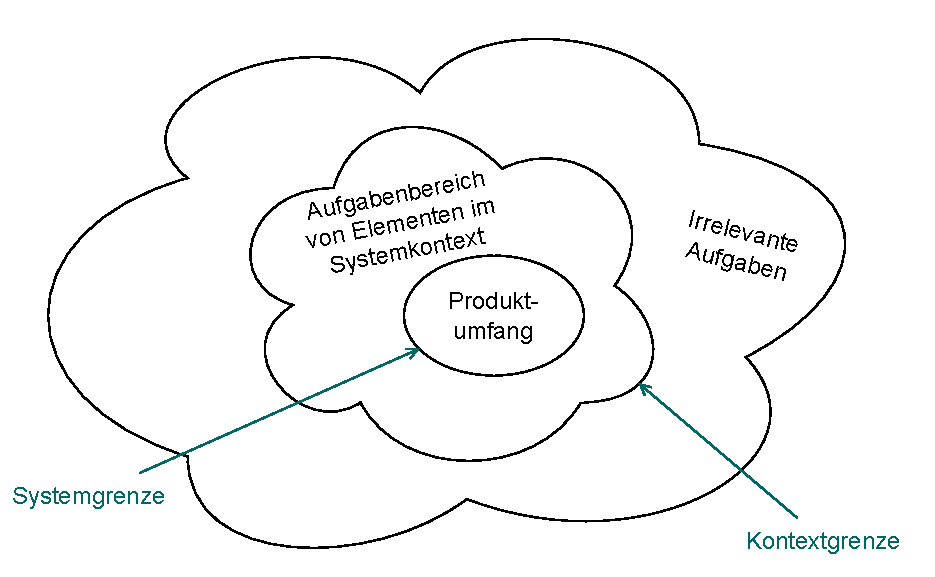
\includegraphics[scale=0.75]{Bilder/Kapitel-6/system-produktumfang.pdf}
	\caption{Aufgabenteilung zwischen dem System und seiner Umgebung}
	\label{fig:system-produktumfang}
	\vspace{\baselineskip} %%% für Druck
\end{figure}

Abbildung~\ref{fig:system-produktumfang} zeigt wieder den Zusammenhang zwischen dem zukünftigen Softwaresystem, seinem Systemkontext und der irrelevanten Umgebung. Diesmal jedoch nicht wie in Abbildung~\ref{fig:system-system} aus einer strukturellen Sicht, sondern aus dem Blickwinkel der Aufgabenverteilung im Betrieb des Softwaresystems. Beschneidet man -- bei gegebener Menge an durchzuführenden Aufgaben -- den Produktumfang des zukünftigen Systems, müssen Elemente des Systemkontexts zusätzliche Aufgaben übernehmen, und umgekehrt. Verschiebt man die Kontextgrenze nach außen, bekommen irrelevante Aufgaben eine Relevanz und müssen von Elementen des Systemkontexts übernommen werden, und umgekehrt.

Der englische Begriff \textit{Scope} für den Produktumfang hat sich im Gegensatz zu den englischen Begriffen Requirements Engineering und Stakeholder in der deutschsprachigen Literatur (noch) nicht durchgesetzt. Wir bleiben daher bei der deutschen Übersetzung, auch wenn der englische Begriff das Konzept besser beschreibt:

\vspace{2mm} %%% für Druck

\begin{itemize}[
	label={\sttpHervorhebung{$\Rightarrow$}},
	]
	\item Das englische Scope kann man außer mit Umfang auch mit Raum, Bereich oder Aufgabenbereich übersetzen. Und die Beschreibung des Produktumfangs besteht eben nicht aus einer Liste der Funktionalitäten des Softwareprodukts, sondern auf einer abstrakteren Ebene aus der Angabe der Aufgabenbereiche, für die das Softwareprodukt zuständig sein soll. Zur Verdeutlichung eine Analogie aus dem Personalverwaltungsbereich: Der Produktumfang entspricht eher einer Arbeitsplatzbeschreibung statt einer Liste der konkreten Arbeits\-tätig\-keiten eines Mitarbeiters.
\end{itemize}

\vspace{2mm} %%% für Druck

Ausgehend vom festgelegten Produktumfang werden konkrete Anforderungen an das zu entwickelnde Softwareprodukt ermittelt. Um hier Ressourcen nicht unnötig zu investieren, sollten die Aufgabenbereiche, die man dem Produktumfang zuordnet, gut durchdacht sein. Das beinhaltet auch die Überlegung, ob sehr verschiedenartige Aufgabenbereiche einfach durch verschiedene Komponenten des späteren Softwaresystems abgedeckt werden oder ob es mehrere eigenständige Produkte geben soll. Im Zoo-Beispiel entwirft Frau Dr. Walther mit ihren ersten vagen Vorstellungen ein Softwareprodukt, das vielfältige Informationen zu den Zootieren bereitstellt, den Besuchern erlaubt, an der Namensgebung der Tiere mitzuwirken, die Übernahme von Tierpatenschaften ermöglicht, die Arbeitsabläufe der Tierpfleger inklusive der Futter\-bestellung verwaltet, die Ausleihe von Tieren und Käfigen aus anderen Zoos unterstützt, die Terminverwaltung der Tierärzte übernimmt und Eintrittskarten für den Zoo verkauft. Bevor man hier den sehr aufwändigen Prozess der Anforderungs\-ermittlung startet, sollte man sich zunächst mit den Stakeholdern darüber verständigen, ob ein einziges Softwareprodukt diese vielen verschiedenen Aufgabenbereiche übernehmen soll oder ob sie Bestandteil unterschiedlicher Software\-entwicklungs\-projekte -- nacheinander oder parallel stattfindend -- sein sollen.

In Softwareentwicklungsprojekten, die nach sequentiellem Vorgehen arbeiten, wird der Produktumfang oft vom Auftraggeber schon vor Start des Softwareentwicklungsprojekts vorgegeben. Der Produktumfang -- und seine Ausdifferenzierung in konkrete Anforderungen -- ist oft auch schon Grundlage des Vertrags zwischen Auftraggeber und Auftragnehmer und im Rahmen des weiteren Softwareentwicklungsprojekts damit nicht mehr grundlegend veränderbar. In agilen Projekten finden durch die stetige Änderungsmöglichkeit im Bereich der Anforderungen automatisch kontinuierliche Verhandlungen zwischen Auftraggeber und Auftragnehmer über den Produkt\-umfang statt. Manche agile Modelle, wie zum Beispiel Extreme Programming, stellen die Notwendigkeit der expliziten Bestimmung des Produktumfangs sogar grundsätzlich in Frage.

\minisec{Rahmenbedingungen}

An dieser Stelle möchten wir noch kurz auf die schon im Kapitel zu Vision und Zielen angesprochenen Rahmenbedingungen zurückkommen. Wir hatten dort zwischen Rahmenbedingungen unterschieden, die in Zusammenhang mit dem Software\-produkt stehen und solchen, die sich auf das Entwicklungsprojekt beziehen. Die produkt\-bezogenen Rahmenbedingungen, wie Gesetze und Richtlinien, die das Softwareprodukt im Betrieb einhalten muss oder die die Architektur des zu entwickelnden Produkts bestimmen, aber auch vorgegebene Hardwareumgebungen für den Betrieb des Systems, sind Elemente des Systemkontexts. Sie werden bei einer systematischen Beschäftigung mit dem Systemkontext während des Entwicklungsprojekts mit berücksichtigt und würden so ihren Weg auch in die Anforderungen finden. Projektbezogene Rahmenbedingungen, wie Zeit- und Kostenbudgets, die zeitliche Verfügbarkeit von Mitarbeitern, die Qualifikation der Mitarbeiter oder auch Möglichkeiten bzw. Unmöglichkeiten Mitarbeiter während des Projekts zu bestimmten Themen fortzubilden, sind nicht Teil des Systemkontexts. Da sie aber entscheidend auf Produktumfang und Systemkontext einwirken können, dürfen sie nicht unberücksichtigt bleiben. Häufig werden sie daher den produktbezogenen Rahmenbedingungen gleichgestellt und als eine besondere Art von Anforderungen (die sogenannten Randbedingungen) behandelt. Wir vertiefen dieses Thema in Abschnitt~\ref{sec:Kap-6.2.2}.